\documentclass{article}

\usepackage{graphicx}
\usepackage{tikz}
\usepackage{tikzsymbols}
\usetikzlibrary{calc,patterns,shapes.geometric}
\pagestyle{empty}
\usepackage[margin=0pt]{geometry}
\geometry{papersize={14in,12in}}

\def\centerarc[#1](#2)(#3:#4:#5){\draw[#1] ($(#2)+({#5*cos(#3)},{#5*sin(#3)})$) arc (#3:#4:#5);}

\begin{document}
	\begin{figure}
		\centering
		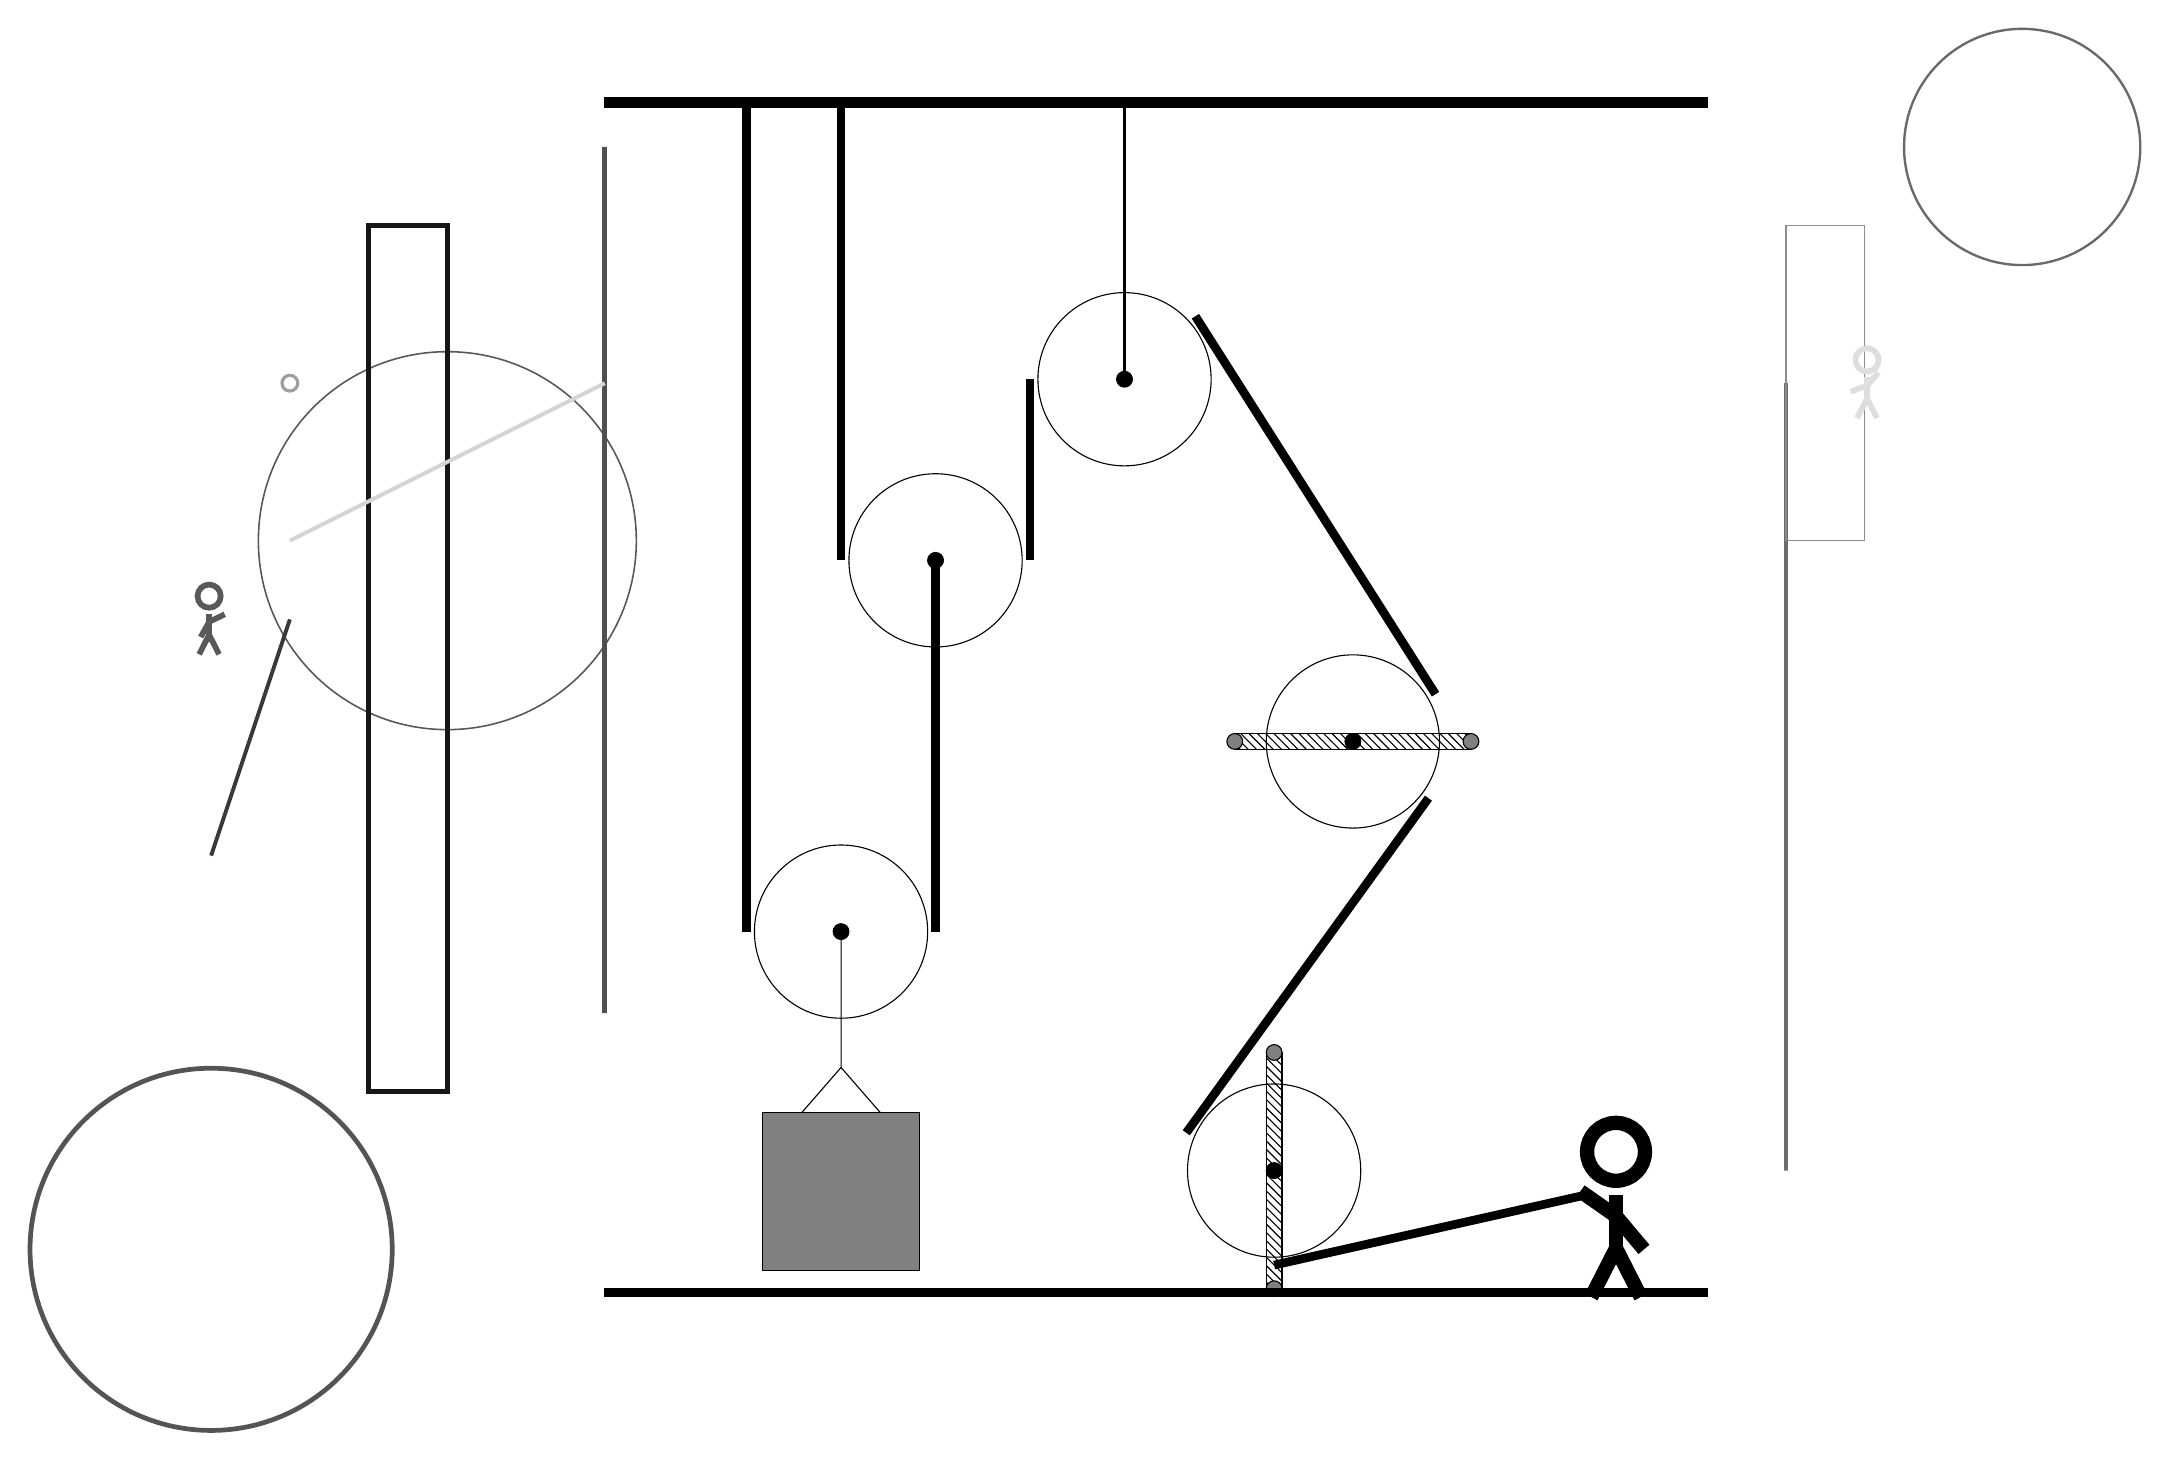
\begin{tikzpicture}
			%%%%% START %%%%%
			
			\draw[fill=black] (-2, 11.5) rectangle (12, 11.625);
			
			\draw (1, 1.035) circle (1.1);
			\draw[fill=black] (1, 1.035) circle (0.1);
			
			\draw (2.2, 5.75) circle (1.1);
			\draw[fill=black] (2.2, 5.75) circle (0.1);
			
			\draw (4.6, 8.05) circle (1.1);
			\draw[fill=black] (4.6, 8.05) circle (0.1);
			\draw[thick] (4.6, 8.05) -- (4.6, 11.5);
			
			\draw (6.5, -2) circle (1.1);
			\draw[fill=black] (6.5, -2) circle (0.1);
			\draw[pattern=north west lines, pattern color=black] (6.4, -0.5) rectangle (6.6, -3.5);
			\draw[fill=black!50] (6.5, -0.5) circle (0.1);
			\draw[fill=black!50] (6.5, -3.5) circle (0.1);
			
			\draw (7.5, 3.45) circle (1.1);
			\draw[fill=black] (7.5, 3.45) circle (0.1);
			\draw[pattern=north west lines, pattern color=black] (6.0, 3.55) rectangle (9.0, 3.35);
			\draw[fill=black!50] (6.0, 3.45) circle (0.1);
			\draw[fill=black!50] (9.0, 3.45) circle (0.1);
			
			\draw (1, 1.035) -- (1, -0.69) -- (0.5, -1.265) -- (1.5, -1.265) -- (1, -0.69);
			\draw[fill=black!50] (0, -1.265) rectangle (2, -3.265);
			
			\draw[line width=1.1mm] (-0.2, 11.5) -- (-0.2, 1.035);
			\centerarc[line width=1.1mm](1, 1.035)(180:360:1.2000000000000002);
			\draw[line width=1.1mm](2.2, 1.035) -- (2.2, 5.75);
			\draw[line width=1.1mm] (1.0, 11.5) -- (1.0, 5.75);
			\centerarc[line width=1.1mm](2.2, 5.75)(180:360:1.2000000000000002);
			\draw[line width=1.1mm](3.4, 5.75) -- (3.4, 8.05);
			\centerarc[line width=1.1mm](4.6, 8.05)(35:180:1.2000000000000002);
			\draw[line width=1.1mm] (5.5, 8.85) -- (8.55, 4.05);
			\centerarc[line width=1.1mm](7.5, 3.45)(215:135:-1.2000000000000002);
			\draw[line width=1.1mm](8.46, 2.73) -- (5.384, -1.52);
			\centerarc[line width=1.1mm](6.5, -2)(-30:100:-1.2000000000000002);
			\draw[line width=1.1mm](6.5, -3.2) -- (10.5, -2.3);
			
			\node at (10.8, -2.5) {\Strichmaxerl[10][-35][-50]};
			
			\draw [line width=0.2mm, color=black!66](-4, 6) circle (2.4);
			
			\draw[line width=0.6mm, color=black!91] (-4, 10) rectangle (-5, -1);
			\draw[line width=0.6mm, color=black!58] (13, -2) rectangle (13, 8);
			\draw[line width=0.5mm, color=black!78](-6, 5) -- (-7, 2);
			\draw [line width=0.6mm, color=black!67](-7, -3) circle (2.3);
			
			\draw [line width=0.4mm, color=black!38](-6, 8) circle (0.1);
			
			\draw[line width=0.2mm, color=black!45] (13, 10) rectangle (14, 6);
			\draw[line width=0.6mm, color=black!69] (-2, 0) rectangle (-2, 11);
			\draw[line width=0.5mm, color=black!17](-2, 8) -- (-6, 6);
			\node[line width=0.3mm, color=black!65] at (-7, 5) {\Strichmaxerl[4][61][26]};
			\node[line width=0.5mm, color=black!13] at (14, 8) {\Strichmaxerl[4][20][49]};
			\draw [line width=0.3mm, color=black!59](16, 11) circle (1.5);
			
			\draw[fill=black] (-2, -3.5) rectangle (12, -3.6);
			
			%%%%% END %%%%%
		\end{tikzpicture}
	\end{figure}	
\end{document}